\documentclass[11pt]{article}
\usepackage[utf8]{inputenc}
\usepackage[T1]{fontenc}
\usepackage[spanish]{babel}
\usepackage{amsmath}
\usepackage{amsfonts}
\usepackage{amssymb}
\usepackage{graphicx}
\usepackage{caption}
\usepackage{wrapfig}
\usepackage{subcaption}
\usepackage{textcomp}
\usepackage{siunitx}
\usepackage{geometry}
\usepackage{courier}
\usepackage{cancel}
\spanishdecimal{.}

\title{Física Numérica}
\author{Julio César Avila Torreblanca}
\date{02 de diciembre del 2021}

\setlength{\parindent}{0cm}
\geometry{verbose,tmargin=1in,bmargin=1in,lmargin=1in,rmargin=1in}
\begin{document}
	\maketitle
	
	\section*{Tarea 7}
	%%%%%%%%%%%%%%%%%%%%%%%%%%%%%%%%%%%%%%%%%%%%%%%%%%%%%%%%%%%%%%%%%%%%%%%%%%%%%%%%%%%%%%%%%%%%%%%%%%%%%%%%%%%%%%%%%%%%%%%%	
	\subsection*{\textbf{1. Ecuación de Poisson}}
	\begin{itemize}
		\item Resuelva numéricamente la ecuación de Poisson:
			$$\frac{\partial^2 \phi}{\partial x^2} + \frac{\partial^2 \phi}{\partial y^2} = f(x,y)$$
			con:
			$$f(x,y) = \cos(3x + 4y) - \cos(5x - 2y)$$
			sujeta a las condiciones de frontera periódica:
			$$\phi (x, 0) = \phi (x,2\pi),\quad \phi (0,y) = \phi(2\pi,y)$$
			Indique el método elegido (Jacobi o Gauss-Seidel), presente su resultado en forma gráfica.
	\end{itemize}
	
	%%%%%%%%%%%%%%%%%%%%%%%%%%%%%%%%%%%%%%%%%%%%%%%%%%%%%%%%%%%%%%%%%%%%%%%%%%%%%%%%%%%%%%%%%%%%%%%%%%%%%%%%%%%%%%%%%%%%%%%%
	\textit{Solución.}\\
	En clase se desarrollo la ecuación de Poisson en 2D de forma numérica:
	$$\nabla^2 \phi (x,y) = -\frac{\rho}{\varepsilon_0}$$
	Llegando a una solución de la forma discretizada:
	$$\phi_{i,j} = \frac{\rho_{i,j}}{4\varepsilon_0} + \frac{1}{4}\left[\phi_{i+1,j} + \phi_{i-1,j} + \phi_{i,j+1} + \phi_{i,j-1}\right]$$
	Para este problema la densidad $\rho$ junto con la constante $\varepsilon_0$ serán sustituidas por la función $f(x,y)$ dada. Además, utilizaremos el método de Gauss-Seidel para obtener la solución. En este método debemos utilizar los últimos valores del potencial calculados. Es decir, que en cada iteración deberemos reescribir los antiguos valores del potencial por los nuevos y con ello la velocidad de convergencia será mayor. Haciendo estos ajustes, nuestra ecuación discretizada nos queda:
	$$\phi_{i,j}^{new} = \frac{1}{4}\left[\phi_{i+1,j}^{old} + \phi_{i-1,j}^{new} + \phi_{i,j+1}^{old} + \phi_{i,j-1}^{new} + f(x,y) \Delta^2 \right]$$
	Donde $\Delta^2 = 2\pi/N$ con $N$ el número de nodos en un lattice de $N\times N$.\\\\
	Para comenzar con el algoritmo requeriremos de las siguientes librerías:
	\begin{figure}[h]
		\centering
		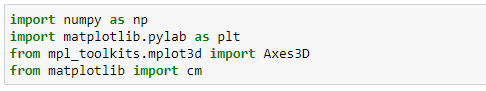
\includegraphics[width=10cm]{Img/1.1.PNG}
	\end{figure}
\newpage
	Lo siguiente a realizar es crear una función que nos calcule la parte $f(x,y) = \cos(3x + 4y) - \cos(5x - 2y)$ en el problema.
	 \begin{figure}[h]
	 	\centering
	 	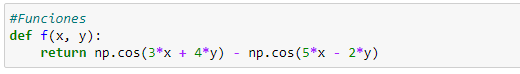
\includegraphics[width=12cm]{Img/1.2.PNG}
	 \end{figure}
 
	Ahora debemos definir dos arreglos de longitud $N$ llenos de números aleatorios. Además, se deben crear dos lattices para ir guardando las soluciones viejas y nuevas. El lattice viejo lo podemos llenar de números aleatorios. Finalmente, se crea otro arreglo donde guardaremos los valores para la función $f(x,y)$.
	\begin{figure}[h!]
		\centering
		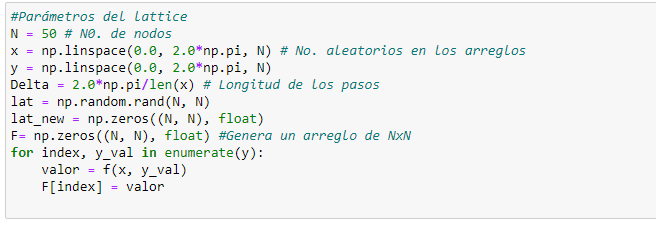
\includegraphics[width=13cm]{Img/1.3.PNG}
	\end{figure}
	
	Ya que tenemos los lattices es necesario establecer nuestras condiciones de frontera al lattice viejo. Nosotros fijaremos estos puntos a $5$ V.
		\begin{figure}[h!]
		\centering
		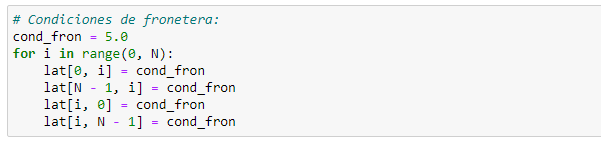
\includegraphics[width=13cm]{Img/1.4.PNG}
	\end{figure}

	Enseguida implementaremos el método de Gauss-Seidel. Para ello es necesario tener un parámetro de tolerancia \texttt{eps} que servirá para comparar punto a punto el lattice nuevo del viejo. Es decir, en cada iteración se obtendrá la diferencia punto a punto del lattice nuevo menos el viejo, y si la diferencia de cada punto es menor a \texttt{eps} habremos terminado con la recursión. Esto se observa en el siguiente algoritmo:
\newpage
	\begin{figure}[h!]
		\centering
		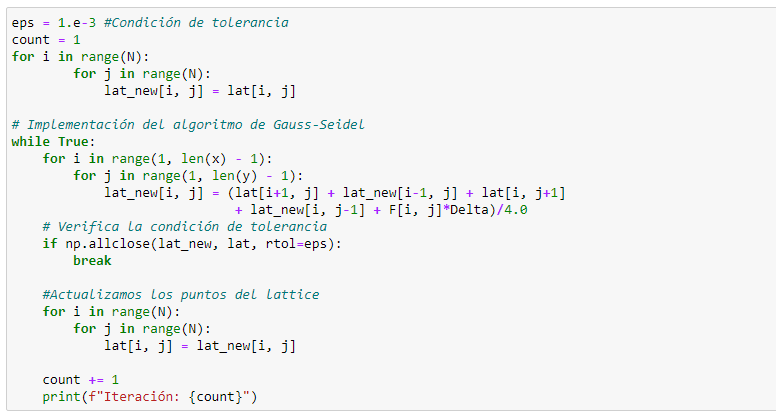
\includegraphics[width=13cm]{Img/1.5.PNG}
	\end{figure}

	Hasta esta parte ya habremos generado el lattice final que contendrá los valores adecuados para nuestra solución. Solo resta determinar las alturas y graficar el resultado.
	\begin{figure}[h!]
		\centering
		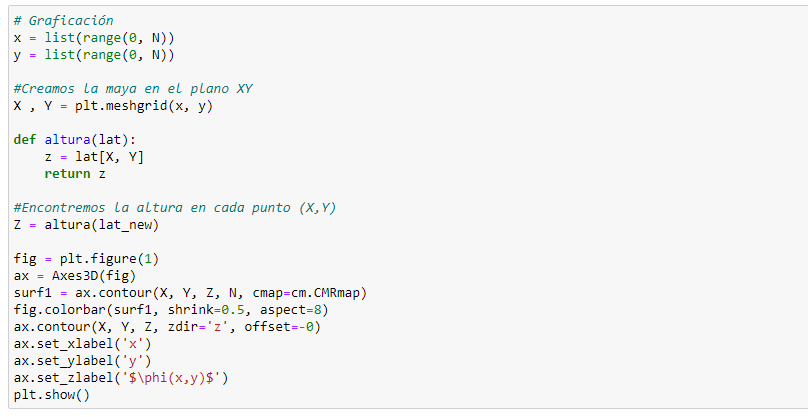
\includegraphics[width=13cm]{Img/1.6.PNG}
	\end{figure}
	
	Como producto final obtenemos:
\newpage
	\begin{figure}[h!]
		\centering
		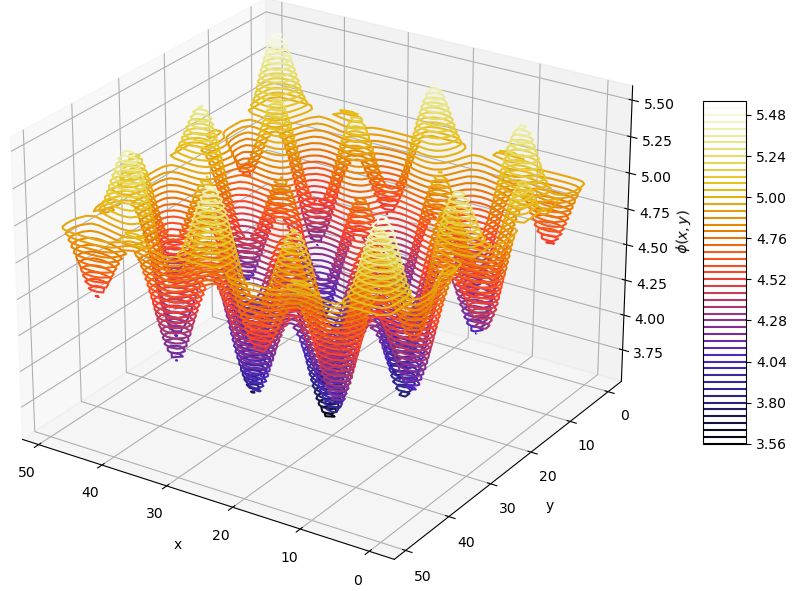
\includegraphics[width=13cm]{Img/1.7.PNG}
		\caption{Solución a la ecuación de Poisson dada.}
	\end{figure}

\hrule
	%%%%%%%%%%%%%%%%%%%%%%%%%%%%%%%%%%%%%%%%%%%%%%%%%%%%%%%%%%%%%%%%%%%%%%%%%%%%%%%%%%%%%%%%%%%%%%%%%%%%%%%%%%%%%%%%%%%%%%%%
	
	\subsection*{\textbf{2. Estados ligados en un potencial arbitrario}}
	\begin{itemize}
	\item Una partícula cuántica en un estado estacionario de energía definida $E$ se encuentra ligada por un potencial $1D$. Su función de onda se determina por la ecuación de Schrödinger independiente del tiempo:
	$$\frac{d^2 \psi (x)}{dx^2} - \frac{2m}{\hbar^2} V(x) \psi (x) = \kappa^2 \psi(x),\quad \kappa^2 = -\frac{2m}{\hbar^2}E$$
	Cuando la partícula está ligada, tenemos que está confinada a cierta región \textit{finita} del espacio, por lo que $\psi(x)$ es normalizable. Esto nos dice que la energía debe ser negativa para que $\psi(x)$ decaiga exponencialmente cunado $x\to \pm \infty$:
	$$\psi (x )\to \left\{\begin{array}{cc}
		e^{-\kappa x},& \text{cuando} x\to +\infty	\\
		e^{+\kappa x},& \text{cuando} x\to -\infty
	\end{array}\right.$$
	Aunque la ecuación puede resolverse con algún método numérico (Runge Kutta, por ejemplo), el extra aquí es que también debemos tener la solución $\psi(x)$ debe satisfacer las condiciones de frontera anteriores. Esta condición adicional convierte al problema de la EDO en un problema de eigenvalores en el cual existe solución solo para ciertos valores del eigenvalor $E$. La solución, si existe, se sigue de encontrar una energía permitida, resolver la ecuación y después variar la energía como parte de un problema de prueba y error (búsqueda de raíces) para la función de onda que satisfaga las condiciones de frontera. 
	\end{itemize}
	%%%%%%%%%%%%%%%%%%%%%%%%%%%%%%%%%%%%%%%%%%%%%%%%%%%%%%%%%%%%%%%%%%%%%%%%%%%%%%%%%%%%%%%%%%%%%%%%%%%%%%%%%%%%%%%%%%%%%%%%\\
\newpage
	\textit{Solución.}\\
	La ecuación que queremos resolver es:
	\begin{equation}
		\frac{d^2 \psi (x)}{dx^2} = \frac{2m}{\hbar^2}\left(V(x) - E\right) \psi (x) 	\label{original}
	\end{equation}
	Donde hemos sustituido el valor de $\kappa$. Notemos que es una EDO de segundo orden, por lo que debemos transformarla usando la forma estándar.\\
	Sean:
	$$y^{(0)} (x) = \psi (x)\quad;\quad y^{(1)}(x) = \frac{d \psi(x)}{dx}$$
	Por lo que:
	\begin{align}
		y^{(1)}(x) &=  \dfrac{dy^{(0)}(x) }{dx}	\label{eq:1}\\
		\frac{dy^{(1)}(x)}{dx} &= \frac{2m}{\hbar^2} (V(x)-E) y^{(0)}(x)	 \label{eq:2}
	\end{align}
	Estas serán las EDO's a resolver en nuestro algoritmo.\\
	Para nuestro programa utilizaremos las siguientes librerías:
	\begin{figure}[h]
		\centering
		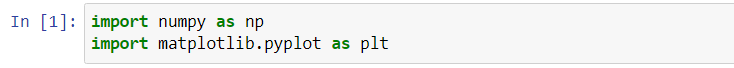
\includegraphics[width=13cm]{Img/2.1.PNG}
	\end{figure}

	En la ecuación (\ref{eq:2}) utilizaremos el siguiente valor para la constante:
	$$\frac{2m}{\hbar^2} = \frac{2mc^2}{(\hbar c)^2} =\frac{2(\SI{0.511}{MeV})}{(\SI{0.197}{MeV\cdot pm})^2}\approx \SI{26.33}{MeV^{-1}pm^{-2}}$$
	Donde hemos usado la masa del electrón $m = \SI{0.511}{MeV/c^2}$. Definimos esta constante en nuestro algoritmo como \texttt{Cte}:
	\begin{figure}[h]
		\centering
		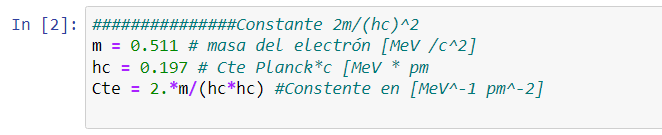
\includegraphics[width=10cm]{Img/2.2.PNG}
	\end{figure}

	Siguiente con el orden sugerido, crearemos una función llamada \texttt{f(x,y)} cuyo propósito es calcular las funciones $f^{(0)}$ y $f^{(1)}$ cuya forma estándar están dadas por:
	\begin{align*}
		f^{(0)} (x) &= y^{(1)} (x)	\\
		f^{(1)} (x) &= \frac{2m}{\hbar^2} (V(x) - E) y^{(0)}
	\end{align*}
	Asumiremos que $E$ está dado. Este valor más adelante se obtendrá por el método de Bisección. La función \texttt{f(x,y)} con su respectiva documentación (comentada) está dada por:
\newpage
	\begin{figure}[h]
		\centering
		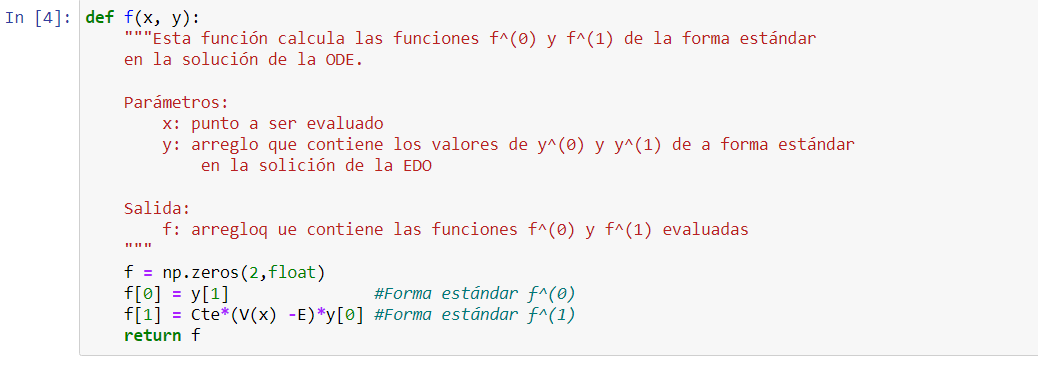
\includegraphics[width=13cm]{Img/2.3.PNG}
	\end{figure}
	
	La función contiene comentarios donde se definen los parámetros y la salida.\\
	Lo siguiente a realizar es definir el potencial $V(x)$. Tomaremos un potencial constante de la siguiente forma:
	\begin{equation}
		V(x) = \left\{\begin{array}{cc}
				-\SI{10}{MeV}, & |x|\leq a	\\
				0 & |x| > a
		\end{array}\right.
	\end{equation}
	Donde consideraremos $a = \SI{10}{pm}$ como la mitad del ancho del pozo, de forma que en el eje $x$ el pozo de potencial finito empieza en $-a$ y termina en $a$. La función que contiene esta parte está dada por:
	\begin{figure}[h]
		\centering
		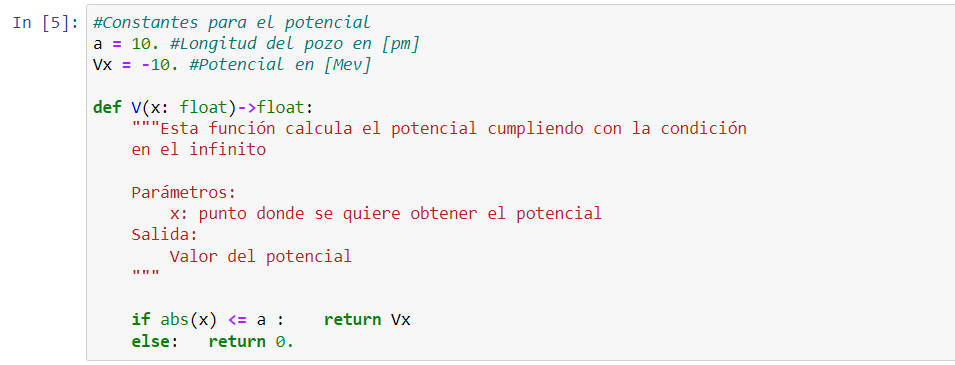
\includegraphics[width=13cm]{Img/2.4.PNG}
	\end{figure}

	Lo que sigue es resolver la EDO, para ello nos apoyaremos del algoritmo de Runge-Kutta de cuarto orden (rk4). Este algoritmo se vio en clase y está dado por:
	\begin{figure}[h]
		\centering
		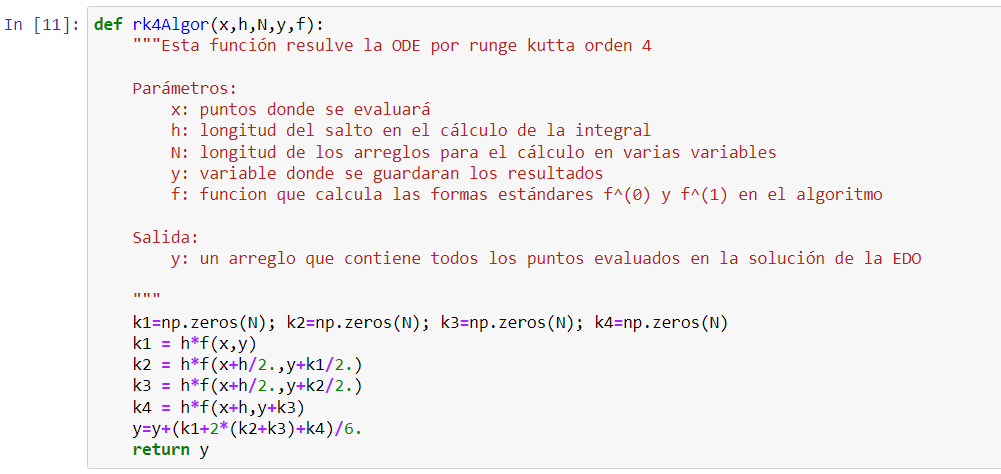
\includegraphics[width=14cm]{Img/2.5.PNG}
	\end{figure}

	Ya con el algoritmo de rk4 procederemos a crear una función llamada \texttt{diff} cuyo objetivo será iniciar la función de onda por izquierda y por derecha en el $X$ que consideraremos como infinito y enseguida se usará el algoritmo de Runge-Kutta para integrar desde el ``infinito'' hasta el punto de pegado y ahí evaluaremos la condición:
	$$\Delta (E,x) =\frac{\frac{\psi_{izq}' (x)}{\psi_{izq} (x)} - \frac{\psi_{dcha}' (x)}{\psi_{dcha} (x)}}{\frac{\psi_{izq}' (x)}{\psi_{izq} (x)} + \frac{\psi_{dcha}' (x)}{\psi_{dcha} (x)}} $$
	
	Tomaremos a $X = 5a$ nuestro infinito ($a$ es la mitad del ancho del pozo). Además, para la función de onda $\psi_{izq}$ por la izquierda en menos infinito consideraremos la aproximación:
	$$\psi_{izq}( x= -X) = e^{-\kappa (x=X)} = e^{-\kappa X}$$
	Por lo que la derivada en ``infinito'' es:
	$$\psi_{izq}'( x = -X) =  \kappa e^{-\kappa X}$$
	En el siguiente fragmento del algoritmo se ve implementada esta primer parte:
	\begin{figure}[h]
		\centering
		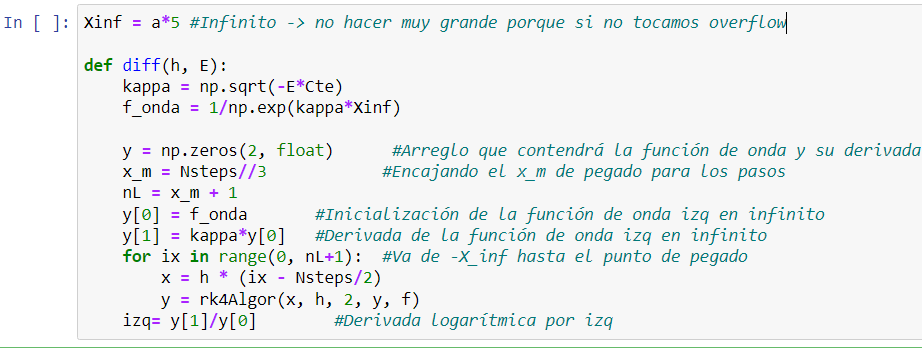
\includegraphics[width=15cm]{Img/2.6.PNG}
	\end{figure}
	
	Notemos que hemos pedido como parámetros la energía $E$ que se encontrará más adelante por bisección y la constante $h$ que contendrá la longitud de los pasos para la integración por Runge-Kutta. Esta parte de la función solo hace el cálculo para la derivada logarítmica $\psi_{izq}'(x)/ \psi_{izq}(x)$ en el punto de pegado. Hace falta calcular por la derecha.\\
	Para la parte derecha es muy similar, solamente que en lugar de integrar hacia delante debemos integrar hacia atrás. Esto lo modificaremos en la función \texttt{rk4Algor} considerando la longitud de paso como $-h$ para ir hacia atrás. Haciendo esta modificación y ajustando el número de pasos para la parte derecha nos queda la función completa como:
\newpage
	\begin{figure}[h]
		\centering
		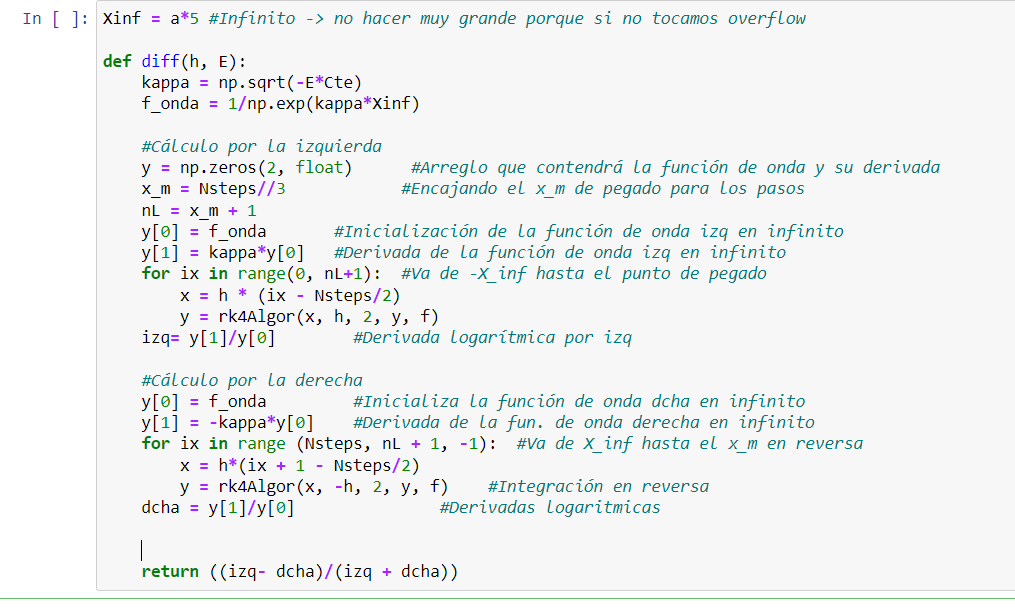
\includegraphics[width=13cm]{Img/2.7.PNG}
	\end{figure}
	 
	 Notemos que la función anterior nos regresa el cálculo de $\Delta (E,x)$ en el punto de pegado. Más adelante buscaremos que este valor sea menor que un $\varepsilon$ dado.\\
	 La siguiente parte que sigue para el algoritmo es generar los calcular las funciones de onda normalizadas por izquierda y por derecha para después pegarlas juntas en un gráfico. La función que calculará estas funciones de onda normalizadas se llamará \texttt{plot(h,E)} con parámetros $h$ la longitud del paso y $E$ la energía. La primer parte de la función que calcula la parte izquierda es la siguiente:
	 \begin{figure}[h]
	 	\centering
	 	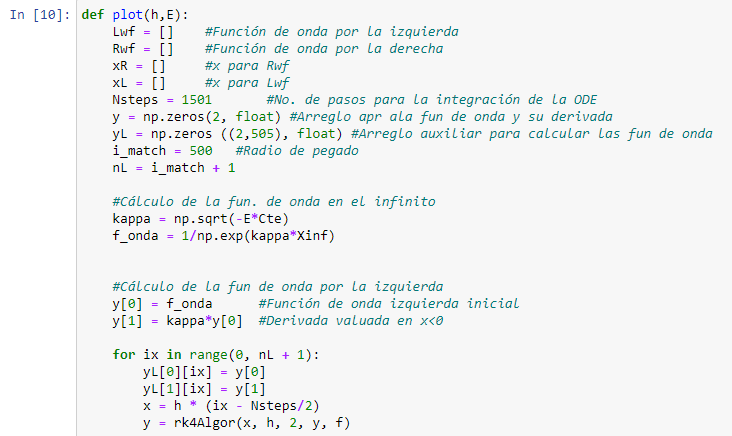
\includegraphics[width=13cm]{Img/2.9.PNG}
	 \end{figure}
 	
 	Dentro de la función se tuvo que generar un arreglo \texttt{yL} auxiliar para guardar los valores de la función de onda izquierda y su derivada. Notemos que este algoritmo es muy parecido al de la función \texttt{diff}, solamente que aquí se usaron más arreglos auxiliares.\\
 	La otra parte de la función está dada por:
\newpage
 	\begin{figure}[h]
 		\centering
 		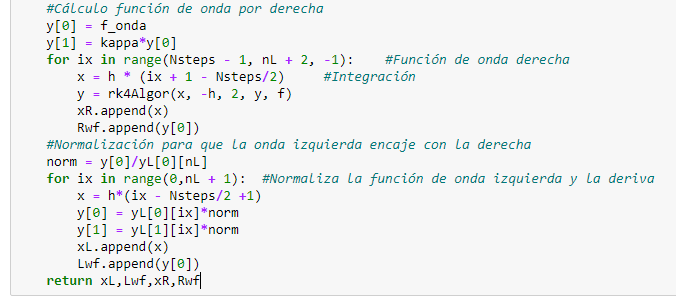
\includegraphics[width=13cm]{Img/2.10.PNG}
 	\end{figure}
 	
 	El cálculo de la onda por la derecha es análogo. Luego, para hacer que coincidiera la onda izquierda y derecha se hizo una normalización para la onda izquierda. Simplemente hay que multiplicar por un factor de escala que contiene a la función de onda por derecha en el punto de pegado entre la función de onda izquierda en el punto de pegado. El algoritmo completo es el siguiente:
 	\begin{figure}[h!]
 		\centering
 		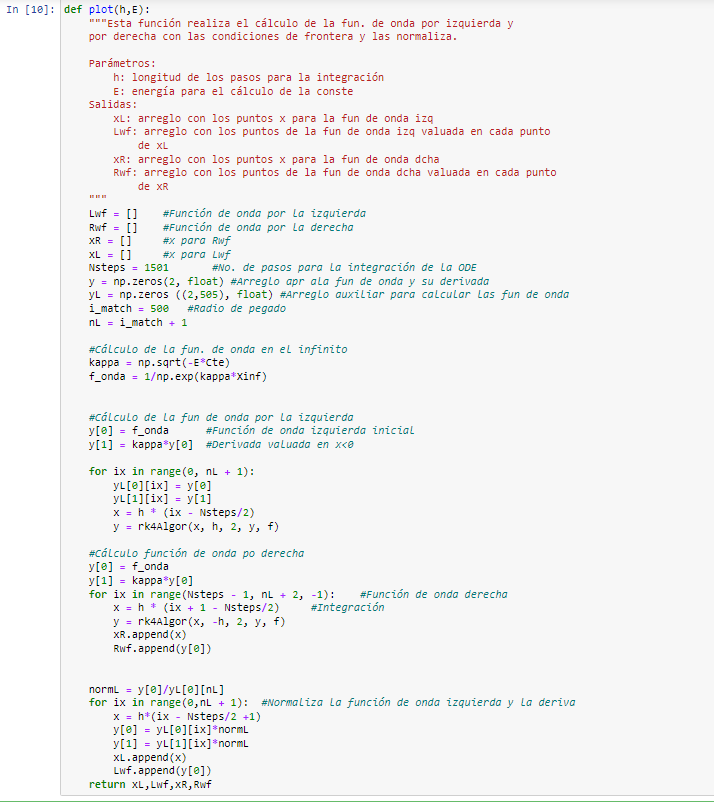
\includegraphics[width=12cm]{Img/2.8.PNG}
 	\end{figure}
 
 	Ya con todas estas funciones podremos realizar la parte central del código donde determinaremos la energía por bisección. En el siguiente algoritmo se realiza la parte de bisección junto con la graficación de cada aproximación obtenida en cada una de las iteraciones.

 	\begin{figure}[h]
 		\centering
 		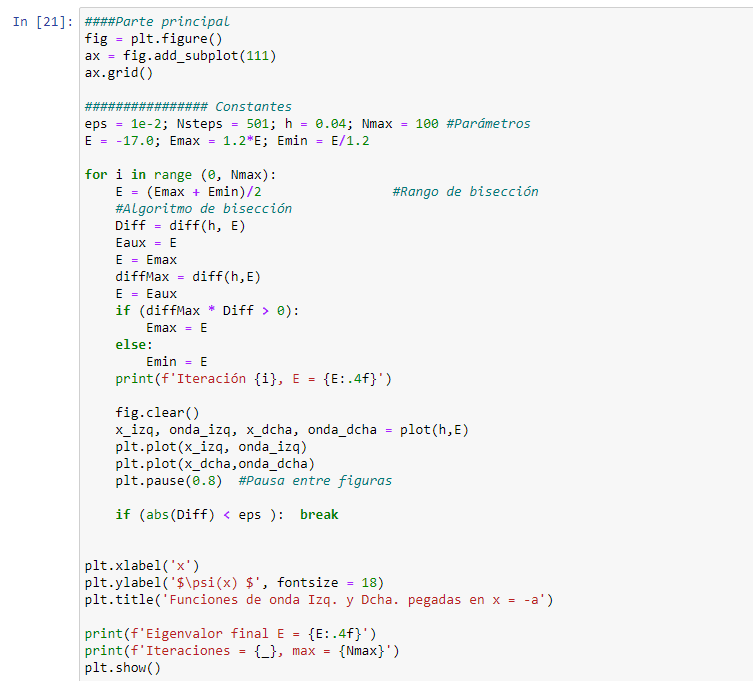
\includegraphics[width=12cm]{Img/2.11.PNG}
 	\end{figure}
 	
 	La variable \texttt{eps} contiene nuestra la tolerancia para la aproximación. Además hemos colocando un número \texttt{Nmax} de iteraciones para no entrar en un bucle infinito si no hay solución. \\
 	La primer parte  del ciclo \texttt{for} contiene la parte del algoritmo de bisección e imprime en cada iteración la energía estimada. Notemos que por sugerencia $|E|< V_0$ para tener una buena aproximación. Así que hay que tener cuidado con esta condición y con los puntos \texttt{Emax} y \texttt{Emin} que contendrán el intervalo donde se realizará el algoritmo de bisección.\\
 	La última parte del algoritmo se encarga crear una gráfica para cada iteración y reescribirla para observar el cambio. Además nos arroja el eigenvalor final para la energía.\\
 	Pongamos a prueba nuestro programa con la siguiente definición de constantes:
 	\begin{figure}[h]
 		\centering
 		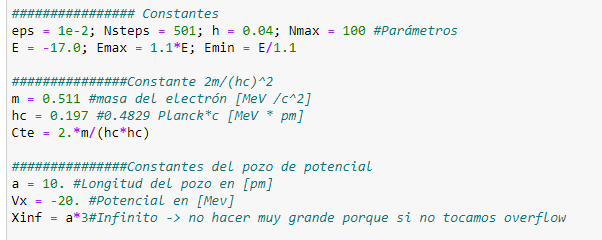
\includegraphics[width=12cm]{Img/2.13.PNG}
 	\end{figure}
 
	Aquí hemos usado la masa de un electrón como ya se mencionó antes. Esto nos produce el siguiente eigenvalor junto con el número de iteraciones:
	\begin{figure}[h]
		\centering
		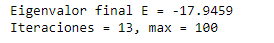
\includegraphics[width=6cm]{Img/2.12.PNG}
	\end{figure}
	
	Y el gráfico final es el siguiente:
	
	\begin{figure}[h]
		\centering
		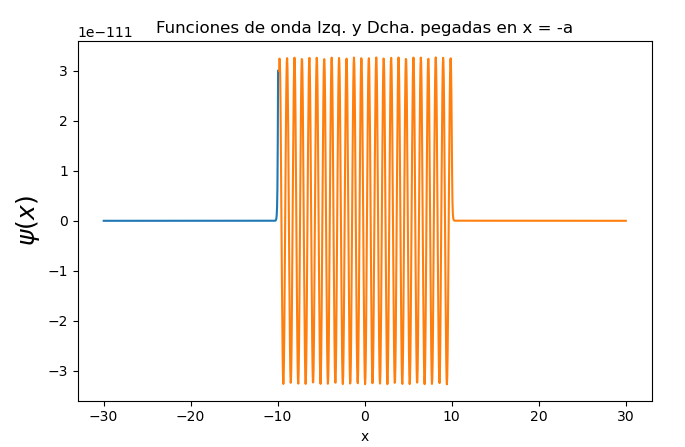
\includegraphics[width=10cm]{Img/2.14.PNG}
	\end{figure}

	Se ve que la función oscila mucho dentro del pozo. Esto se debe a que hemos considerado la masa del electrón. Si modificamos el valor de la variable \texttt{Cte} en nuestro algoritmo por \texttt{Cte}$=0.4829$ (un valor relativamente adecuado) obtenemos el siguiente resultado para el eigenvalor:
	\begin{figure}[h]
		\centering
		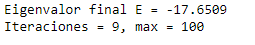
\includegraphics[width=6cm]{Img/2.15.PNG}
	\end{figure}
	
	Y para la solución gráfica:
	\begin{figure}[h!]
		\centering
		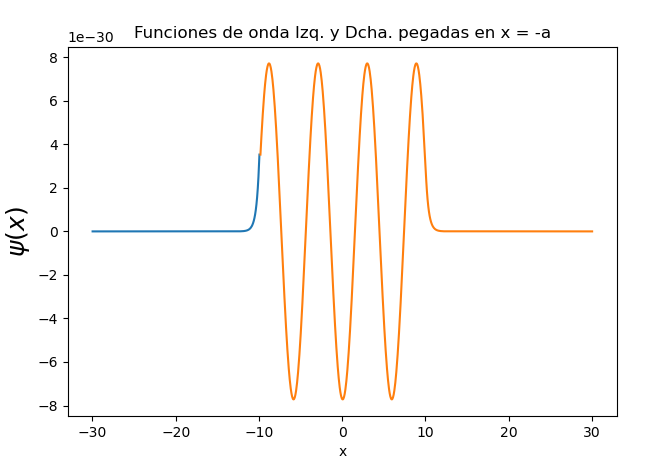
\includegraphics[width=10cm]{Img/2.16.PNG}
	\end{figure}
	
	En esta última se aprecia mucho mejor el comportamiento de la función de onda.
	%%%%%%%%%%%%%%%%%%%%%%%%%%%%%%%%%%%%%%%%%%%%%%%%%%%%%%%%%%%%%%%%%%%%%%%%%%%%%%%%%%%%%%%%%%%%%%%%%%%%%%%%%%%%%%%%%%%%%%%%
	
	
	
	
	
	
	
	
	
	
\end{document}